\chapter{The Analysis of the Utah Parolee Data}

The statistical analysis of recidivism among parolees released from state prison in Utah is presented in this chapter.  The first section describes the survey instrument, the sampling methodology, the data cleaning process, the choice of predictor variables, and the descriptive statistics of the parolees.  A brief discussion of the statistical modeling techniques used is found in the second section.  The results of the statistical analyses are contained in sections 5.3 through 5.5.  The statistical analysis focuses upon the use of two Bayesian techniques:  Bayesian Model Averaging and Classification and Regression Trees.  These techniques are were chosen to address the issues of model specification uncertainty and nonhomogeneous relationships in the data, respectively. The analysis centers upon identifying which variables belong to the best model of recidivism and comparing the effectiveness of economic and noneconomic variables as predictors of recidivism.  Section 5.6 contains the generalizations of the analysis.

\section{The survey and descriptive statistics}

The Utah 2006 Census of Parolees served as the primary source of the data used in this analysis.  Upon testing the survey instrument, the survey was administered to all of the Utah parolees that reported to their parole officers during the third week of May, 2006.  All parolees in Utah are required to report on a monthly basis, which implies that approximately one-fourth of Utah's parolees were surveyed.  The assignment of reporting dates to parolees within any month appears to be completely arbitrary, suggesting a high likelihood that the sample is perfectly random. The response rate to the survey was 100\%.  Given the large size of the sample relative to the population, its apparent randomness, and the 100\% response rate, it can be confidently asserted that the sample is an unbiased, representative sample of the Utah parolee population.

Two versions of a questionnaire were used, one for the employed and one for the unemployed.  The information gathered falls into three broad categories:  demographic, educational, and economic.  The demographic information collected included age and race.  The educational information gathered included educational attainment (GED, high school diploma, college degree, and vocational certificate) and participation in prison educational programs (GED, high school, postsecondary, or none).  The economic information can be separated into two categories:  work-related information and information about the parolee's living conditions.  For employed parolees, data was collected on their hourly wage, hours worked per week, occupation, receipt of health benefits, and employment at a second job.  Unemployed parolees were asked about reasons for not having a job, time spent looking for employment, methods used to find employment, and type of work sought.  With respect to living conditions, information was gathered from all parolees regarding rent, number of people living in the household, and the receipt of assistance for rental payments.  All parolees were also asked if they owned a car.  Finally, information was collected for all parolees on restitution payments, child support payments, and the amounts of the payments in each case.

The information gathered from the survey was combined with information provided by the Utah Department of Corrections. The data from the Utah Department of Corrections included information on gender, number of prior incarcerations, type of crime for which the parolee was most recently incarcerated, and returns to prison after May 2006.  These two sources provided all of the data used in the analysis below.

Data was collected from 760 parolees.  However, not all of the initial 760 observations were usable for the statistical analyses.  Three-year follow-up information was only available for 666 of the initial 760 observations.  This was due to the parolee either not indicating his or her Utah State Prison (USP) number or incorrectly recording the number.  Incorrect USP numbers were detected when matching the survey data to the corrections data and these individuals were eliminated.  Another 18 observations were eliminated because the individual in each case either died and was not reimprisoned, was never previously imprisoned, or was imprisoned during the period at which the survey was administered.  In the latter two cases, these are likely the results of parolees incorrectly recording their USP numbers.  This further reduced the number of usable observations to 648.

Additional observations were excluded due to missing values in the data set.  At this point in the process, personal judgment enters as a choice must be made between the trade-off of either removing observations or removing variables from the data set.  Some variables were considered crucial to the analysis, while others had to be eliminated for the sake of maintaining the number of observations.  Very few parolees had second jobs, so all of the variables related to having a second job were excluded.  Likewise, all of the living conditions variables were left out because there were many missing values.  Finally, the variables recording the amounts for restitution and child support payments were also eliminated due to the large number of missing values.  However, the dummy variables for restitution and child support variables were retained.  After eliminating the variables mentioned above and excluding all observations with missing values, 506 observations remained for use in the data analyses.

%----- Note that the table reference is below the table.

\begin{table}[h]
\begin{center}
\caption{Descriptive Statistics for Utah Parolees}
\vspace{0.1cm}
\small
\begin{tabular}{lr@{.}lr@{.}lr@{.}lr@{.}l}
  \hline
  Variable & \multicolumn{2}{c}{Minimum} & \multicolumn{2}{c}{Maximum} & \multicolumn{2}{c}{Mean} & \multicolumn{2}{c}{Median} \\ \hline
  Age at time of survey & \hspace{0.25cm} 20 & 58 & \hspace{0.25cm} 74 & 92 & 36 & 87 & \ \ 35 & 66 \\
  Male                 &    & 00 &  1 & 00 &    & 86 &  1 & 00 \\
  African American     &    & 00 &  1 & 00 &    & 06 &    & 00 \\
  Asian                &    & 00 &  1 & 00 &    & 01 &    & 00 \\
  Hispanic             &    & 00 &  1 & 00 &    & 15 &    & 00 \\
  Native American      &    & 00 &  1 & 00 &    & 02 &    & 00 \\
  Pacific Islander     &    & 00 &  1 & 00 &    & 02 &    & 00 \\
  White                &    & 00 &  1 & 00 &    & 73 &  1 & 00 \\
  Prior Incarcerations &  1 & 00 &  9 & 00 &  1 & 98 &  1 & 00 \\
  Most recent crime: Driving      &    & 00 &  1 & 00 &    & 06 &    & 00 \\
  Most recent crime: Drug offense &    & 00 &  1 & 00 &    & 25 &    & 00 \\
  Most recent crime: Murder       &    & 00 &  1 & 00 &    & 03 &    & 00 \\
  Most recent crime: Other        &    & 00 &  1 & 00 &    & 02 &    & 00 \\
  Most recent crime: Person       &    & 00 &  1 & 00 &    & 17 &    & 00 \\
  Most recent crime: Property     &    & 00 &  1 & 00 &    & 27 &    & 00 \\
  Most recent crime: Sex offense  &    & 00 &  1 & 00 &    & 20 &    & 00 \\
  Most recent crime: Weapons      &    & 00 &  1 & 00 &    & 01 &    & 00 \\
  GED                                 &    & 00 &  1 & 00 &    & 36 &    & 00 \\
  High school diploma                 &    & 00 &  1 & 00 &    & 71 &  1 & 00 \\
  College degree                      &    & 00 &  1 & 00 &    & 09 &    & 00 \\
  Vocational certificate              &    & 00 &  1 & 00 &    & 21 &    & 00 \\
  Prison education: None              &    & 00 &  1 & 00 &    & 27 &    & 00 \\
  Prison education: GED               &    & 00 &  1 & 00 &    & 23 &    & 00 \\
  Prison education: High school       &    & 00 &  1 & 00 &    & 50 &  1 & 00 \\
  Prison education: Post-secondary    &    & 00 &  1 & 00 &    & 30 &    & 00 \\
  Employed                  &    & 00 &  1 & 00 &    & 76 &  1 & 00 \\
  Hours per week            &    & 00 & 84 & 00 & 29 & 85 & 40 & 00 \\
  Wage                      &    & 00 & 47 & 00 &  8 & 08 &  8 & 50 \\
  Health benefits           &    & 00 &  1 & 00 &    & 26 &    & 00 \\
  Job type: Management      &    & 00 &  1 & 00 &    & 05 &    & 00 \\
  Job type: Building        &    & 00 &  1 & 00 &    & 04 &    & 00 \\
  Job type: Sales           &    & 00 &  1 & 00 &    & 07 &    & 00 \\
  Job type: Office          &    & 00 &  1 & 00 &    & 11 &    & 00 \\
  Job type: Construction    &    & 00 &  1 & 00 &    & 30 &    & 00 \\
  Job type: Installation    &    & 00 &  1 & 00 &    & 10 &    & 00 \\
  Job type: Production      &    & 00 &  1 & 00 &    & 12 &    & 00 \\
  Job type: Transportation  &    & 00 &  1 & 00 &    & 07 &    & 00 \\
  Restitution payments      &    & 00 &  1 & 00 &    & 50 &  1 & 00 \\
  Child support payments    &    & 00 &  1 & 00 &    & 33 &    & 00 \\
  Car ownership             &    & 00 &  1 & 00 &    & 42 &    & 00 \\
  \hline
\end{tabular}
\end{center}
\end{table}

The descriptive statistics for the 506 observations are produced in Table 5.1.  A few of the variables are in need of some additional explanation as their use in the modeling process required special coding.  For the wage and the hours worked per week variables, these were coded as 0 for those who were unemployed.  As a result, the mean values for these variables in Table 5.1 are lower than the mean values for only those who were employed.  For the 383 parolees who were employed, their mean wage was \$10.67 and their mean number of hours worked per week was 39.4.  The job type variables also require some clarification.  There are eight job types, all of which are dummy variables, but their sum equals 86\% of the data.  This is higher than the percentage of those employed (76\%) because it was possible that some parolees held more than one job.

The descriptive statistics and their interpretations for the remaining variables are straightforward.  The  sociological variables are discussed first.  Of the 506 parolees in the final data set, the average age was 36 and 86\% were male.  The race dummy variables exclude those who did not respond, so the sum will equal 100\% of the data.  Whites (73\%) and Hispanics (15\%) were the largest groups.  Every parolee had at least one prior conviction and the average was two prior convictions.  Regarding the last crime for which the individual was incarcerated, the two most common crimes were property crimes (27\%) and drug-related crimes (25\%).  The least frequent crimes were weapons-related (1\%), other crimes (2\%), and murder (3\%).

Turning to the educational variables, 71\% of the parolees had a high school diploma and 9\% had a college degree (the latter variable includes 2-year associates degrees).  Approximately 50\% attended high school courses while in prison, 30\% attended postsecondary courses, and 27\% did not participate in prison educational programs at all.  It should be noted that both the educational attainment and prison education categories are not mutually exclusive.  Thus, the variables GED, high school diploma, college degree, and vocational certificate sum to greater than 100\%.  The same is true for the prison education variables GED, high school, post-secondary, and none.

The only economic variables not mentioned thus far are health benefits, restitution payments, and child support payments.  The health benefits variable specifically measures employer-provided health care benefits.  For those who were employed, 34.5\% received benefits.  Roughly half of the 506 parolees made restitution payments and one-third made child support payments.

Finally, a few words should be devoted to characterizing the recidivism variable.  Recidivism was measured as any return to prison, whether a new crime or technical violation, during the 3-year period after the survey was administered.  Of the 506 parolees used in the final data set, 221 returned at least once to prison.  This yields a 3-year reincarceration rate of 43.8\% for Utah.  For the purpose of comparison, the 3-year reincarceration rate, based on both new crimes and technical violations, is 51.8\% for the United States (Langan \& Levin, 2002).  Figure 5.1 shows the percentage of parolees reincarcerated over the 3-year period.  The shape of the graph is very typical as compared to those from other recidivism studies.  It is a well-established fact that the largest number of offender who do return to prison will do so during the first year, with a smaller percentage returning each subsequent year.  Using more precise terminology, the recidivism rate can be describe as increasing as a decreasing rate.

\begin{figure}[b]
\begin{center}
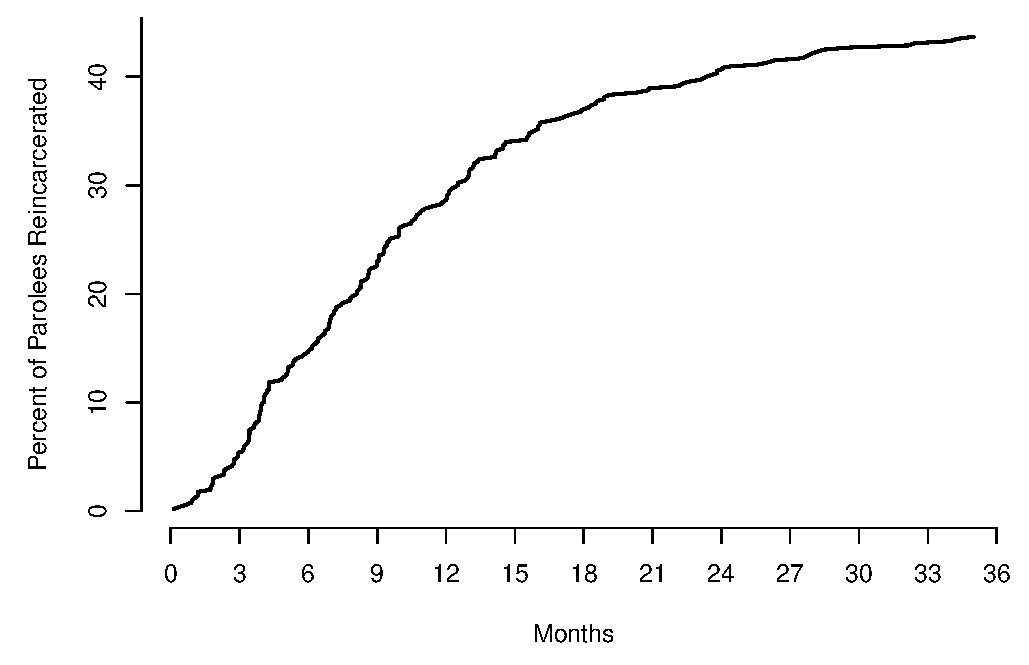
\includegraphics[scale=0.8]{graph531.eps}
\caption{Utah Parolee Recidivism Over Time}
\end{center}
\end{figure}

\section{The statistical methodology}

For the prediction of recidivism, the relevant type of model is one designed to predict the value of a binary dependent variable.  The basic set of standard models used to predict binary dependent variables includes the linear probability model, the logit model, and the probit model.  While one of the standard techniques is used here to model the data, the central focus rests upon two Bayesian modeling techniques.  The only standard model used to analyze the Utah parolee data is a linear probability model and it is included strictly for the purpose of comparison.  Besides the traditional criticisms of the linear probability model, which include predicted probability values great than one or less than zero and inherent heteroskedasticity, there are more serious difficulties that cannot be solved by this modeling technique.  In and of itself, a classical linear regression (CLR) model estimated using ordinary least squares (OLS) offers no guidance regarding the issue of model specification uncertainty.  Once the analyst chooses a set of independent variables, an OLS regression estimates the coefficients as if the specification is, in fact, the best model.  Although there are tests designed to detect specification errors in CLR OLS models (e.g., omitted variable and RESET tests), they are designed to signal that the model is misspecified without indicating where the error lies.  One of the Bayesian methods used in the analysis is specifically directed toward this problem.

A second difficulty involves modeling nonhomogeneous relationships within the data.  An OLS regression estimates coefficients using every observation in the data set, which forces it to ignore differences in a relationship across the range of the data.  It is true that linear regression models can deal with misspecified functional form through creative data transformations, but, for data sets with large numbers of predictors, potentially hundreds of new variables may result.  This, in turn, only exacerbates the model selection problem.  The other Bayesian technique used here specifically addresses the problem of nonhomogeneous relationships in the data.

The statistical analysis of the data centers upon two Bayesian techniques.  The first technique is Bayesian Model Averaging (BMA) and its importance is in addressing the two problems of model specification uncertainty and coefficient magnitude uncertainty.  This technique is fundamentally important to the analysis of recidivism because there is no consensus on the specification of the best recidivism model.  Tests such as the omitted variable and RESET tests give only a general indication that a model might be misspecified and they point to unknown variables outside of the model.  The BMA approach to model specification uncertainty is quite different.  BMA calculates posterior distributions for each of the coefficients so that a probability can be assigned to each variable indicating the likelihood that it is a predictor in the best model.  It is in this way that it addresses model specification uncertainty.  The method also takes into consideration uncertainty regarding the size of the coefficient.  If a variable is included in a model and it is less than certain that it belongs to the best model, the estimated coefficient should reflect that uncertainty.  BMA addresses this issue by adjusting the coefficients in accordance with their probabilities of being members of the best model.

The second Bayesian technique used here is Classification and Regression Tree (CART) analysis.  The tree models produced by this method are easy to interpret and use in comparison to standard regression output.  More importantly, the CART method can produce tree models that fit the data better and offer more accurate predictions by exploiting nonhomogeneous relationships in the data.  An OLS regression operates on only the entire range of values for the variables and does not take into account changes in the relationships across the ranges of the data.  A tree model is essentially a set of conditional statements, which make this a fundamentally Bayesian approach.  The conditional statements that determine the branching of a tree model effectively separate the data into subsets.  Each subset may reveal new relationships among the variables that were not discernable at the level of the entire data set. Subsequent branches are formed by selecting new conditional statements based on these new relationships that separate the data in a way that improves prediction.  Thus, the CART method effectively addresses the issue of nonhomogeneous relationships, an issue that presents significant difficulties for OLS regression models.

\section{Bayesian Model Averaging}

\subsection{Introduction and theoretical overview}

To motivate the problem of model specification uncertainty, note that the Utah parolee data set contains 37 independent variables.  This implies that there are more than 137 billion possible model specifications, or exactly $2^{37}$ possible models.  In order to give a sense of the magnitude of this number in terms of computation time, consider that there are approximately 31.5 billion seconds in 1,000 years. Thus, it is impossible for any individual to compute and visually inspect 137 billion OLS linear regressions in a lifetime.  Stepwise methods for finding the best model, whether bottom-up or top-down, are extremely risky, if not altogether unreliable.  At any step in the process, the elimination of a single variable may dramatically change the $t$ statistics and magnitudes for the remaining coefficients, thereby creating a false impression of which variables belong to the best model.  A coefficient may have a low $t$ statistic for only 1\% of the entire set of models, but if the stepwise procedure begins inside that 1\% the variable will likely be discarded from all future consideration.  BMA effectively addresses this problem by exhaustively searching for the best model specifications and using those models to assign probabilities to the independent variables indicating their likelihood of being members of the best model.

As its name suggests, BMA is a technique that examines a large set of the most-likely models and estimates averaged coefficients based on the frequency with which the variables are selected along with the magnitudes of the coefficients in each case.  Model combining and model averaging were studied as early as the 1960s, but it was not until 1978 that Edward Leamer fully elaborated the ideas that would eventually develop into Bayesian Model Averaging (Hoeting, Madigan, Raftery, \& Volinsky, 1999).  BMA became practical in the mid-1990s only after several theoretical and computational advances.  Raftery, Madigan, and Hoeting (1997) and Hoeting et al. (1999) provide theoretical discussions of BMA and the following theoretical overview is based on these two sources.

The fundamental concept in BMA is the calculation of probability distributions for each of the coefficients based the probability distributions for the coefficients in each of the selected models and the probabilities associated with each model's being the best model.  Let $\mathcal{M}$ represent the set of $k$ possible models:  $\mathcal{M} = \{M_1, \ldots, M_k \}$.  If $\Delta$ is some quantity of interest, such as a coefficient for a linear regression, the posterior distribution of $\Delta$ given the data, $D$, is defined as

\begin{equation}
\mbox{Pr}(\Delta | D) = \sum_{k=1}^K \mbox{Pr}(\Delta | D, M_k) \mbox{Pr}(M_k|D).
\end{equation}

The posterior distribution in Equation (5.1) represents a weighted average of the probability distributions for $\Delta$ for each model $k$, where the weight is the probability that model $k$ is the true model.  It is assumed that the true model is encompassed by the $k$ models so that $\sum_k \mbox{Pr}(M_k|D)=1$.  The posterior model probability for model $k$ is defined as

\begin{equation}
\mbox{Pr}(M_k|D) = \frac{\mbox{Pr}(D|M_k) \mbox{Pr}(M_k)}{\sum_{l=1}^K \mbox{Pr}(D|M_l)\mbox{Pr}(M_l)}.
\end{equation}

Equation (5.2) is an application of Bayes's Theorem to the issue of model uncertainty.  The posterior probability for model $k$ will be proportional to the prior distribution for model $k$, Pr$(M_k)$, times the integrated likelihood function for model $k$, which is given in Equation (5.3).

\begin{equation}
\mbox{Pr}(D|M_k) = \int \mbox{Pr}(D|\theta_k, M_k)\mbox{Pr}(\theta_k|M_k) d\theta_k
\end{equation}

For large data sets with many independent variables, a completely exhaustive calculation of Equation (5.1) for all variables is not practical.  Instead, a smaller subset of models having the highest posterior model probabilities is selected.  There are three methods generally used to determine the subset of the best models:  Occam's window, the leaps and bounds algorithm, and Markov chain Monte Carlo model composition.  The BMA models for the Utah parolee data were fitted using the statistical software R.  Model selection was performed using the leaps and bounds algorithm, so only this method is described.

The leaps and bounds algorithm was developed by Furnival and Wilson (1974) specifically for addressing the model selection problem when given large data sets.  The goal is to identify the best independent variables in terms of their predictive accuracy on the basis of having the smallest residual sum of squares (RSS).  The method relies upon the fact that if $A$ is a model where the variables are a subset of the variables in model $B$, then $\mbox{RSS}(B)\leq \mbox{RSS}(A)$.  An appropriately chosen branching method can be used to exhaust all of the possible models given an initial set of variables.  An initial lower bound can be found by randomly selecting a single variable and calculating its RSS.  A first wave of subsets (i.e., model specifications) is selected and the RSS is calculated for each subset.  For those subsets with an RSS greater than the initial lower bound, they can be ignored because none of the variables in that subset can have a lower RSS than that for the initial variable.  For those subsets with an RSS lower than the initial bound, the subset is branched to form additional subsets and the RSS is calculated for each new subset.  Once a variable is found with a lower RSS than the initial lower bound, this lower RSS becomes the new lower bound.  This process greatly reduces the time needed to find the best model specifications by skipping over those sets of model specifications that cannot possibly have variables with the lowest RSS.

In addition to the problem of finding the subset of the best models, another difficulty in applying BMA is integrating the likelihood function in (5.3).  This can be approximated using the Bayesian Information Criterion (BIC).  For linear regressions, the BIC function is defined as

\begin{equation}
\mbox{BIC}_k = n\log(1-R^2_k)+p_k\log n.
\end{equation}

In equation (5.4), $R^2_k$ is the R-squared for the $k$th model, $p_k$ is the number of regressors in the $k$th model, and $n$ is the number of observations in the data set. The higher the $R^2_k$ score, the lower is the BIC score.  Naturally, those models with the lowest BIC scores are considered the best models.  A low BIC score, or a high $R^2$ score, means that the model fits the data relatively well, which will produce a relatively high $\mbox{Pr}(D|M_k)$ in Equation (5.3).  This, in turn, implies that the posterior model probability, $\mbox{Pr}(M_k|D)$ in Equation (5.2), will likewise be relatively high.  Thus, there will be a natural correspondence between how well a particular model predicts the data and its posterior model probability of being the best model.

\subsection{Results of the analysis}

BMA was applied to the Utah parolee data set to predict returns to prison using 37 independent variables.  The averaging process was applied to an underlying linear probability model structure.  Although prior probabilities can be assigned to each of the variables, no prior probabilities were assumed.  Thus, the data were left to ``speak for themselves.''  A few variables were removed before running the analysis. The hours worked per week variable was removed because of high collinearity with the employment variable ($r=.9$).  The race variable ``White'' was removed to avoid perfect collinearity, so all race coefficients can be interpreted as relative to Whites.  Likewise, the crime type ``other'' was excluded to avoid perfect collinearity, so all crime type coefficients can be interpreted as relative to other crimes.  The results of the BMA analysis are presented in Table 5.2.

\begin{table}[t]
\begin{center}
\caption{Bayesian Model Averaging Coefficient Estimation}
\vspace{0.1cm}
\footnotesize
\begin{tabular}{lr@{.}lr@{.}lr@{.}lr@{.}lr@{.}lr@{.}lr@{.}lr@{.}l}
  \hline
  \multicolumn{17}{l}{74 models were selected}  \\
  \multicolumn{17}{l}{Best  5  models (cumulative posterior probability =  0.1907 ):}  \\ \hline
  & \multicolumn{2}{c}{$p\neq 0$} & \multicolumn{2}{c}{\ \ EV} & \multicolumn{2}{c}{ \ SD} & \multicolumn{2}{c}{\ \ $M_1$} & \multicolumn{2}{c}{\ \ $M_2$} & \multicolumn{2}{c}{\ \ $M_3$} & \multicolumn{2}{c}{\ \ $M_4$} & \multicolumn{2}{c}{\ \ $M_5$} \\ \hline
intercept    & 100 & 0 &   & 643 &   & 134 &   & 662 &   & 709 &   & 684 &   & 725 &   & 678 \\
age          &  79 & 0 &$-$& 005 &   & 003 &$-$& 007 &$-$& 007 &$-$& 007 &$-$& 007 &$-$& 007 \\
male         &     & 0 &   & 000 &   & 000 & \multicolumn{2}{c}{\ \ $\cdot$} & \multicolumn{2}{c}{\ \ $\cdot$} & \multicolumn{2}{c}{\ \ $\cdot$} & \multicolumn{2}{c}{\ \ $\cdot$} & \multicolumn{2}{c}{\ \ $\cdot$} \\
priorinc    &  92 & 8 &   & 045 &   & 020 &   & 053 &   & 049 &   & 049 &   & 048 &   & 052 \\
hispanic     &     & 0 &   & 000 &   & 000 & \multicolumn{2}{c}{\ \ $\cdot$} & \multicolumn{2}{c}{\ \ $\cdot$} & \multicolumn{2}{c}{\ \ $\cdot$} & \multicolumn{2}{c}{\ \ $\cdot$} & \multicolumn{2}{c}{\ \ $\cdot$} \\
pacisland  &     & 0 &   & 000 &   & 000 & \multicolumn{2}{c}{\ \ $\cdot$} & \multicolumn{2}{c}{\ \ $\cdot$} & \multicolumn{2}{c}{\ \ $\cdot$} & \multicolumn{2}{c}{\ \ $\cdot$} & \multicolumn{2}{c}{\ \ $\cdot$} \\
natamer    &     & 0 &   & 000 &   & 000 & \multicolumn{2}{c}{\ \ $\cdot$} & \multicolumn{2}{c}{\ \ $\cdot$} & \multicolumn{2}{c}{\ \ $\cdot$} & \multicolumn{2}{c}{\ \ $\cdot$} & \multicolumn{2}{c}{\ \ $\cdot$} \\
aframer    &  56 & 5 &   & 129 &   & 132 &   & 229 &   & 225 &   & 230   & \multicolumn{2}{c}{\ \ $\cdot$} & \multicolumn{2}{c}{\ \ $\cdot$} \\
asian        &  57 & 2 &$-$& 287 &   & 289 &$-$& 518 &$-$& 488  & \multicolumn{2}{c}{\ \ $\cdot$} &$-$& 501 &$-$& 532 \\
drug      &     & 0 &   & 000 &   & 000 & \multicolumn{2}{c}{\ \ $\cdot$} & \multicolumn{2}{c}{\ \ $\cdot$} & \multicolumn{2}{c}{\ \ $\cdot$} & \multicolumn{2}{c}{\ \ $\cdot$} & \multicolumn{2}{c}{\ \ $\cdot$} \\
driving     &     & 0 &   & 000 &   & 000 & \multicolumn{2}{c}{\ \ $\cdot$} & \multicolumn{2}{c}{\ \ $\cdot$} & \multicolumn{2}{c}{\ \ $\cdot$} & \multicolumn{2}{c}{\ \ $\cdot$} & \multicolumn{2}{c}{\ \ $\cdot$} \\
murder    &     & 0 &   & 000 &   & 000 & \multicolumn{2}{c}{\ \ $\cdot$} & \multicolumn{2}{c}{\ \ $\cdot$} & \multicolumn{2}{c}{\ \ $\cdot$} & \multicolumn{2}{c}{\ \ $\cdot$} & \multicolumn{2}{c}{\ \ $\cdot$} \\
person    &   8 & 5 &$-$& 011 &   & 040 & \multicolumn{2}{c}{\ \ $\cdot$} & \multicolumn{2}{c}{\ \ $\cdot$} & \multicolumn{2}{c}{\ \ $\cdot$} & \multicolumn{2}{c}{\ \ $\cdot$} & \multicolumn{2}{c}{\ \ $\cdot$} \\
property      &  33 & 0 &   & 043 &   & 067 & \multicolumn{2}{c}{\ \ $\cdot$} & & 129 &   & 133 &   & 134  & \multicolumn{2}{c}{\ \ $\cdot$} \\
sexcrime       &   3 & 6 &$-$& 006 &   & 031 & \multicolumn{2}{c}{\ \ $\cdot$} & \multicolumn{2}{c}{\ \ $\cdot$} & \multicolumn{2}{c}{\ \ $\cdot$} & \multicolumn{2}{c}{\ \ $\cdot$} & \multicolumn{2}{c}{\ \ $\cdot$} \\
weapons   &     & 0 &   & 000 &   & 000 & \multicolumn{2}{c}{\ \ $\cdot$} & \multicolumn{2}{c}{\ \ $\cdot$} & \multicolumn{2}{c}{\ \ $\cdot$} & \multicolumn{2}{c}{\ \ $\cdot$} & \multicolumn{2}{c}{\ \ $\cdot$} \\
highsch &   2 & 5 &$-$& 003 &   & 018 & \multicolumn{2}{c}{\ \ $\cdot$} & \multicolumn{2}{c}{\ \ $\cdot$} & \multicolumn{2}{c}{\ \ $\cdot$} & \multicolumn{2}{c}{\ \ $\cdot$} & \multicolumn{2}{c}{\ \ $\cdot$} \\
ged          &     & 0 &   & 000 &   & 000 & \multicolumn{2}{c}{\ \ $\cdot$} & \multicolumn{2}{c}{\ \ $\cdot$} & \multicolumn{2}{c}{\ \ $\cdot$} & \multicolumn{2}{c}{\ \ $\cdot$} & \multicolumn{2}{c}{\ \ $\cdot$} \\
college  &     & 0 &   & 000 &   & 000 & \multicolumn{2}{c}{\ \ $\cdot$} & \multicolumn{2}{c}{\ \ $\cdot$} & \multicolumn{2}{c}{\ \ $\cdot$} & \multicolumn{2}{c}{\ \ $\cdot$} & \multicolumn{2}{c}{\ \ $\cdot$} \\
vocation     &     & 0 &   & 000 &   & 000 & \multicolumn{2}{c}{\ \ $\cdot$} & \multicolumn{2}{c}{\ \ $\cdot$} & \multicolumn{2}{c}{\ \ $\cdot$} & \multicolumn{2}{c}{\ \ $\cdot$} & \multicolumn{2}{c}{\ \ $\cdot$} \\
pednone      &     & 0 &   & 000 &   & 000 & \multicolumn{2}{c}{\ \ $\cdot$} & \multicolumn{2}{c}{\ \ $\cdot$} & \multicolumn{2}{c}{\ \ $\cdot$} & \multicolumn{2}{c}{\ \ $\cdot$} & \multicolumn{2}{c}{\ \ $\cdot$} \\
pedged       &  14 & 0 &$-$& 016 &   & 043 & \multicolumn{2}{c}{\ \ $\cdot$} & \multicolumn{2}{c}{\ \ $\cdot$} & \multicolumn{2}{c}{\ \ $\cdot$} & \multicolumn{2}{c}{\ \ $\cdot$} & \multicolumn{2}{c}{\ \ $\cdot$} \\
pedhs        &     & 0 &   & 000 &   & 000 & \multicolumn{2}{c}{\ \ $\cdot$} & \multicolumn{2}{c}{\ \ $\cdot$} & \multicolumn{2}{c}{\ \ $\cdot$} & \multicolumn{2}{c}{\ \ $\cdot$} & \multicolumn{2}{c}{\ \ $\cdot$} \\
pedpost        &     & 0 &   & 000 &   & 000 & \multicolumn{2}{c}{\ \ $\cdot$} & \multicolumn{2}{c}{\ \ $\cdot$} & \multicolumn{2}{c}{\ \ $\cdot$} & \multicolumn{2}{c}{\ \ $\cdot$} & \multicolumn{2}{c}{\ \ $\cdot$} \\
employed     & 100 & 0 &$-$& 200 &   & 050 &$-$& 200 &$-$& 193 &$-$& 191 &$-$& 201 &$-$& 208 \\
wage         &     & 0 &   & 000 &   & 000 & \multicolumn{2}{c}{\ \ $\cdot$} & \multicolumn{2}{c}{\ \ $\cdot$} & \multicolumn{2}{c}{\ \ $\cdot$} & \multicolumn{2}{c}{\ \ $\cdot$} & \multicolumn{2}{c}{\ \ $\cdot$} \\
healthben   &     & 0 &   & 000 &   & 000 & \multicolumn{2}{c}{\ \ $\cdot$} & \multicolumn{2}{c}{\ \ $\cdot$} & \multicolumn{2}{c}{\ \ $\cdot$} & \multicolumn{2}{c}{\ \ $\cdot$} & \multicolumn{2}{c}{\ \ $\cdot$} \\
managejob    &     & 0 &   & 000 &   & 000 & \multicolumn{2}{c}{\ \ $\cdot$} & \multicolumn{2}{c}{\ \ $\cdot$} & \multicolumn{2}{c}{\ \ $\cdot$} & \multicolumn{2}{c}{\ \ $\cdot$} & \multicolumn{2}{c}{\ \ $\cdot$} \\
buildjob    &     & 0 &   & 000 &   & 000 & \multicolumn{2}{c}{\ \ $\cdot$} & \multicolumn{2}{c}{\ \ $\cdot$} & \multicolumn{2}{c}{\ \ $\cdot$} & \multicolumn{2}{c}{\ \ $\cdot$} & \multicolumn{2}{c}{\ \ $\cdot$} \\
salesjob    &     & 0 &   & 000 &   & 000 & \multicolumn{2}{c}{\ \ $\cdot$} & \multicolumn{2}{c}{\ \ $\cdot$} & \multicolumn{2}{c}{\ \ $\cdot$} & \multicolumn{2}{c}{\ \ $\cdot$} & \multicolumn{2}{c}{\ \ $\cdot$} \\
officejob   &     & 0 &   & 000 &   & 000 & \multicolumn{2}{c}{\ \ $\cdot$} & \multicolumn{2}{c}{\ \ $\cdot$} & \multicolumn{2}{c}{\ \ $\cdot$} & \multicolumn{2}{c}{\ \ $\cdot$} & \multicolumn{2}{c}{\ \ $\cdot$} \\
constrjob   &     & 0 &   & 000 &   & 000 & \multicolumn{2}{c}{\ \ $\cdot$} & \multicolumn{2}{c}{\ \ $\cdot$} & \multicolumn{2}{c}{\ \ $\cdot$} & \multicolumn{2}{c}{\ \ $\cdot$} & \multicolumn{2}{c}{\ \ $\cdot$} \\
installjob  &     & 0 &   & 000 &   & 000 & \multicolumn{2}{c}{\ \ $\cdot$} & \multicolumn{2}{c}{\ \ $\cdot$} & \multicolumn{2}{c}{\ \ $\cdot$} & \multicolumn{2}{c}{\ \ $\cdot$} & \multicolumn{2}{c}{\ \ $\cdot$} \\
prodjob     &     & 0 &   & 000 &   & 000 & \multicolumn{2}{c}{\ \ $\cdot$} & \multicolumn{2}{c}{\ \ $\cdot$} & \multicolumn{2}{c}{\ \ $\cdot$} & \multicolumn{2}{c}{\ \ $\cdot$} & \multicolumn{2}{c}{\ \ $\cdot$} \\
transjob    &     & 0 &   & 000 &   & 000 & \multicolumn{2}{c}{\ \ $\cdot$} & \multicolumn{2}{c}{\ \ $\cdot$} & \multicolumn{2}{c}{\ \ $\cdot$} & \multicolumn{2}{c}{\ \ $\cdot$} & \multicolumn{2}{c}{\ \ $\cdot$} \\
restitution  &  61 & 4 &   & 074 &   & 068 &   & 118 & \multicolumn{2}{c}{\ \ $\cdot$} & \multicolumn{2}{c}{\ \ $\cdot$}  &  \multicolumn{2}{c}{\ \ $\cdot$}  &   & 121 \\
childsup   &  38 & 2 &   & 042 &   & 061 & \multicolumn{2}{c}{\ \ $\cdot$} & \multicolumn{2}{c}{\ \ $\cdot$} & \multicolumn{2}{c}{\ \ $\cdot$} & \multicolumn{2}{c}{\ \ $\cdot$} & \multicolumn{2}{c}{\ \ $\cdot$} \\
owncar      &  27 & 4 &$-$& 030 &   & 054 & \multicolumn{2}{c}{\ \ $\cdot$} & \multicolumn{2}{c}{\ \ $\cdot$} & \multicolumn{2}{c}{\ \ $\cdot$} & \multicolumn{2}{c}{\ \ $\cdot$} & \multicolumn{2}{c}{\ \ $\cdot$} \\ \hline
\multicolumn{7}{l}{Number of Variables} & \multicolumn{2}{c}{\ \ 6} & \multicolumn{2}{c}{\ \ 6} & \multicolumn{2}{c}{\ \ 5} &  \multicolumn{2}{c}{\ \ 5} & \multicolumn{2}{c}{\ \ 5} \\
\multicolumn{7}{l}{$R^2$} &  & 109 & & 108 & & 097 & & 097 & & 097 \\
\multicolumn{7}{l}{BIC} & -20 & 948 & -20 & 749 & -20 & 625 & -20 & 569 & -20 & 535 \\
\multicolumn{7}{l}{Posterior probability} & & 043 & & 039 & & 037 & & 036 & & 035 \\
  \hline
\end{tabular}
\normalsize
\end{center}
\end{table}

In Table 5.2, ``$p\neq 0$'' denotes the probability that the coefficient is not zero, ``EV'' represents the expected value of the coefficient, and ``SD'' is the standard deviation for the coefficient.  The leaps and bounds algorithm selected the 74 best models, five of which are produced in the table.  The five models in the table are sorted from smallest to highest BIC score, which corresponds to the models being ``most likely correct'' to ``least likely correct.''  This correspondence is also reflected in the posterior model probabilities given in the last line in Table 5.2 for the five best models.

Turning to the results for each variable, the discussion separates the variables into the categories of economic and noneconomic variables.  Beginning with the economic variables, the single-most important variable for predicting recidivism is employment.  With a posterior probability of 100, the employment variable certainly belongs to the best model of recidivism.  The absolute value of the coefficient is the second largest among all coefficient, implying it has a large effect on recidivism.  If a parolee is employed, it reduces the probability of returning to prison by 20 percentage points relative to an unemployed parolee.  The second most important economic variable is restitution.  With a posterior probability of 61.4\%, this variable is very likely a member of the best model.  If a parolee pays restitution, the probability of returning to prison increases 7.4 percentage points.  The child support variable is the only other economic variable with strong results.  The posterior probability of 38.2\% indicates that, while not dominant, the child support variable has a significant role to play in predicting recidivism.  The probability of returning to prison increases by 4.2 percentage points when a parolee must pay child support. The wage variable appears unimportant and this is because it is highly collinear with the employment variable ($r=.79$).  In the presence of high collinearity, BMA typically selects one variable and ignores the other.  Health benefits and occupational type do not appear to be important predictors of recidivism.

The educational variables do not appear to be strong predictors of recidivism.  One possible explanation is that because offenders must report felonies on employment applications, the effects of education on employment status and the wage rate are suppressed.  Of all of the educational variables, only the educational attainment variable for high school diploma and the prison education variable for GED preparation have some importance.  In both cases, they slightly reduce the probability of returning to prison.

As for the noneconomic variables, the number of prior incarcerations is the strongest predictor with a posterior probability of 92.8\%.  For each prior incarceration, a parolee is 4.5 percentage points more likely to return to prison.  With a posterior probability of 79\%, age at the time of the survey is the next strongest predictor of recidivism.  For each additional year in age, the probability of returning to prison drops by $.5$ percentage points.  Two race variables were also important predictors.  The Asian variable has a posterior probability of 57.2\% and the African American variable has a posterior probability of 56.5\%, which makes both of these variables important.  The probability of an Asian parolee returning to prison is 28.7 percentage points lower than for a White parolee, while the probability of returning to prison for an African American parolee is 12.9 percentage points higher than a White parolee.  The last variable of importance is the type of crime most recently committed before the survey was administered.  The property crime variable has a 33\% probability of being in the best model.  If a parolee's most recent conviction was for a property crime, the probability of returning to prison is 4.3 percentage points higher in comparison to those in the ``other crime'' category.

The method by which the posterior probabilities for the coefficients are determined is graphically represented in Figure 5.2.  All 74 of the best models are listed along the horizontal axis in order of ``most likely correct'' to ``least likely correct.''  For each model, the variables included in that model are indicated by the black bars.  The determination of the posterior probability for a coefficient will depend on the number of times the variable is used  weighted by the model's ranking in which it is used.


\begin{figure}[t]
\begin{center}
\includegraphics[clip=true,viewport=0mm 0mm 168mm 180mm, scale=0.85]{graph521.eps}
\caption{Models Selected by Bayesian Model Averaging}
\end{center}
\end{figure}

The usefulness of Figure 5.2. lies in the fact that the values found under the ``$p\neq 0$'' column of Table 5.2 are presented in such a way that the relative importance of each variable can be easily visualized and understood.  For instance, employment status is the most important predictor of recidivism and, with a posterior probability of 100, it is certainly a member of the best model.  Correspondingly, a solid black bar traverses the entire range of the 74 best models indicating its inclusion in every model.  The next two strongest predictors of recidivism are prior incarcerations and age, and the black bars representing their inclusion in the models reveal only a small number of gaps where they were not included.  The restitution variable is the fourth strongest predictor and its importance can be seen by its inclusion in the majority of the models.  Likewise, the importance of the child support variable and the Asian and African American race variables can be immediately perceived.

A few comments regarding the fit of the BMA model deserve mention.  Using the data to evaluate the fit of the BMA model, the model correctly classifies 64.8\% of parolees.  The model predicts that 149 of the parolees will return to prison, whereas 221 actually returned.

\subsection{A 10-fold cross-validation of three recidivism models}

Of central importance to this dissertation is the determination of the relative importance of economic variables in predicting recidivism versus noneconomic variables.  Information regarding noneconomic variables, such as age, race, and gender, is collected as a matter of policy by corrections departments and, as a result, is relatively inexpensive to obtain.  Economic information, on the other hand, is more costly to acquire.  Thus, the collection of economic data on parolees and probationers is only justified in so far as it leads to a better understanding of those factors that increase the risk of recidivism.

In order to determine the relative importance of economic variables in predicting recidivism, a 10-fold cross-validation of three models is performed.  The three models used in this experiment are referred to as the Sociological Model, the Economic Model, and the Total Model.  The Sociological Model includes only those variables that are sociological in nature and can be easily obtained from any corrections department.  These variables include age, gender, race, prior incarcerations, and most recent crime committed.  The Economic Model is based solely on the variables for employment, restitution, and child support.  The Total Model uses all of the variables.  The results for the three models are found in Table 5.3.

\begin{sidewaystable}
\begin{center}
\caption{Results of Three 10-Fold Cross-Validations}
\vspace{0.1cm}
\begin{tabular}{lccccccccccc}
  \hline
  \multicolumn{12}{c}{Correct Classifications} \\ \hline
 Fold & 1 & 2 & 3 & 4 & 5 & 6 & 7 & 8 & 9 & 10 & Overall \\ \hline
 Sociological Model & .5098 & .5686 & .6078 & .5882 & .6471 & .6078 & .6275 & .5098 & .5882 & .5686 & .5824 \\
 Economic Model & .5490 & .5686 & .5490 & .6471 & .6078 & .6275 & .6078 & .5098 & .6275 & .5686 & .5863 \\
 Total Model & .5490 & .6078 & .6078 & .7451 & .6667 & .5882 & .6275 & .5294 & .5882 & .5882 & .6098 \\ \hline
 \multicolumn{12}{c}{Mean Square Error} \\ \hline
 Fold & 1 & 2 & 3 & 4 & 5 & 6 & 7 & 8 & 9 & 10 & Overall \\ \hline
 Sociological Model & .2396 & .2377 & .2474 & .2212 & .2324 & .2277 & .2427 & .2619 & .2380 & .2420 & .2391 \\
 Economic Model & .2430 & .2435 & .2404 & .2204 & .2237 & .2484 & .2242 & .2588 & .2175 & .2334 & .2353 \\
 Total Model & .2513 & .2418 & .2574 & .2171 & .2232 & .2350 & .2259 & .2621 & .2339 & .2537 & .2402 \\
\hline
\end{tabular}
\end{center}
\end{sidewaystable}

The 10-fold cross-validation was performed by randomly sorting the data and dividing it into 10 more-or-less equal subsets.  Each subset contained 51 observations and two subsets had four observations in common.  For the three models, 90\% of the data was used as training data for estimating the coefficients, then the model was used to predict the remaining 10\%.  This was performed systematically so that predictions were made for each of the 10 subsets based on the other 90\% of the data.  Thus, every observation served as training data and testing data for all three models.  For each model, BMA was used to estimate the coefficients for a linear probability model using only those variables included in the model and excluding all other variables.  Naturally, the Total Model uses all of the variables.  Two measures were used to evaluate predictive accuracy.  The first measure is the number of correct classifications over the total number of 51 predictions, which essentially produces a ratio of successes.  The second measure is the mean square error, which measures how close the predicted value is to the actual value.

Looking across the folds, each model performs relatively better than some other model for a given fold and relatively worse in another fold.  The last column gives the overall results as averages for the 10 folds for each model.  The Economic Model, which used only the three variables of employment, restitution, and child support, correctly classified parolees slightly better than the Sociological Model.  When all of the information was used, the Total Model produced a correct classification rate approximately 2.5 percentage points higher than the other two models.  The Economic Model had the lowest mean square error, which implies that the predicted and actual values were closer on average than for the other two models.  The results suggest that economic variables are just slightly better predictors of recidivism than sociological variables.  Furthermore, when both economic and sociological variables are used together, the correct classification rate can be improved significantly.

\section{Classification and Regression Trees}

While the use of trees for classification and regression dates back to the 1960s, the first complete, formal treatment of tree methodology was produced by Breiman, Friedman, Olshen, and Stone (1984).  The CART method encompasses two types of models.  A classification tree is used to model an equation where the response variable is a categorical variable and a regression tree is used for a numerical response variable.  As the interest here lies with predicting a binary categorical variable (i.e., return to prison), the models developed here are classification trees.

Tree methodology has several advantages over other methods of statistical classification.  Because tree models are easy to interpret, they can be implemented within practical settings by individuals with essentially no statistical background.  Furthermore, the informational and computational requirements for classifying observations through the use of a tree are minimal.  A regression equation requires knowledge of all values of the variables and often involves considerable computation in order to determine the class membership of an observation.  A tree, on the other hand, can typically classify a large number of observations using only a few variables and, in some cases, the necessary computations are reduced to determining the values of binary variables.  More importantly, the tree methodology offers an effective method for treating nonhomogeneous relationships.  A classification tree is essentially a series of conditional statements and these conditional statements divide observations into subsets corresponding to the different qualities of the nonhomogeneous relationship (e.g., the observations determining a quadratic relationship can be divided into those exhibiting a positive relationship and those exhibiting a negative relationship).  Not only can a classification tree reveal information about nonhomogeneous relationships within the data simply through its structure, but it will tend to better fit the data and produce more accurate predictions when taking account of nonhomogeneous relationships as compared to linear classification methods.

The tree models found in this dissertation were produced using the statistical software R.  The characterization of the tree construction process follows Breiman et al. (1984).  Forming a classification tree involves three aspects:  determining the splitting rules, deciding when to stop splitting nodes, and assigning terminal nodes to classes.  When selecting a splitting rule for a node, the goal is to choose an independent variable and a split point such that the observations are separated into two subsets, each of which is \emph{purer} than the predecessor set.  The notion of \emph{purity} is defined formally in terms of an impurity function $i(t)$, where $i( \cdot )$ is a nonnegative function measuring the impurity at node $t$.  The function $i(t)$ will be at its largest value when all of the class types are mixed together and the function will be zero for some node when its only members are of one class.  In terms of the prisoner recidivism problem, the data set of 506 parolees contains 43.7\% who returned to prison and 56.3\% who did not.  For this initial node, the impurity function $i(t)$ would be at its maximum.  If it were possible to completely separate those who returned from those who did not, the function $i(t)$ would be zero at each of the two terminal nodes containing the 221 who returned and the 285 who did not.

The impurity function is ultimately used to determine the best independent variable and the best split point along the range of that variable for a splitting rule at a particular node.  Large data sets can produce millions of possible splitting rule and some criterion must be used to find the best rule.  Numerical variables can theoretically produce an infinite number of splitting rules, but for practical purposes only several thousand split points might be considered.   Binary categorical variables will only have one possible split point.  Let $\mathcal{S}$ denote the set of all possible splits corresponding to all of the independent variables and all of their split points, where $s$ denotes an individual split such that $s \in \mathcal{S}$.  Breiman et al. (1984) define the goodness of the split $s$ as the decrease in impurity measured by the function

\begin{equation}
\Delta i(s, t) = i(t) - p_L \cdot i(t_L) - p_R \cdot i(t_R),
\end{equation}

\noindent where $t$ is the initial node, $t_L$ and $t_R$ are the left and right successor nodes, $p_L$ is the proportion of observations in node $t_L$ taken from $t$, and $p_R$ is the proportion of observations in node $t_R$ taken from $t$.  Each split $s$ will have a corresponding measure of goodness.  Finally, the best splitting rule $s^*$ for some node $t$ is determined as the one that produces the greatest reduction in impurity and is defined as

\begin{equation}
\Delta i (s^*, t) = \max_{s \in \mathcal{S}} \Delta i(s, t).
\end{equation}

Given the nature of the splitting method, those splits that occur earlier in the tree construction process usually indicate variables that are stronger predictors of the dependent variable.  Once the best split $s^*$ has been determined for the initial node, the splitting procedure is performed anew on each of the successor nodes, and so on.  The way in which the tree methodology treats nonhomogeneous relationships can be understood in relationship to the splitting method described above.  Assuming two independent variables $x_1$ and $x_2$, it might be that no clear relationships between either $x_1$ or $x_2$ and the dependent variable $y$ can be perceived when examining linear regression output or even scatterplots of the data.  When constructing a tree, if a split occurs using the variable $x_1$, the resulting subsets in the successor nodes may exhibit very strong relationships between $x_2$ and $y$.  This conditional approach to modeling the data essentially reveals relationships that may exist only within subsets and not at the level of the entire data set.  Because linear regression models only operate at the level of the entire data set, they cannot detect relationships that occur only within subsets of the data (i.e., nonhomogeneous relationships).

Turning to the Utah parolee data, two classification trees were modeled on the data.  Both are interpreted as follows.  Observations that satisfy the splitting rule at a given node are classified to the left branch and those that do not satisfy the rule are classified to the right.  The vertical length of a branch connecting two nodes indicates the importance of the variable at the predecessor node.  The longer the branch, the greater is the decrease in impurity.  The probability for each terminal node is calculated as the number of parolees that returned to prison divided by the total number of parolees in the terminal node.  If the probability at the terminal node is greater than or equal to $.5$, then all parolees classified to that terminal node are predicted to return to prison within three years.  Nodes with probabilities less than $.5$ determine sets of parolees that are predicted not to return to prison.

The best tree model, CART Model 1, is presented in Figure 5.3.  The tree was constructed using the same data set as was used for the BMA model with the exception that the wage variable was removed.  The data set contains 506 observations and 36 independent variables.  The model predicts that a total of 194 of the 506 parolees from the data set will return to prison within three years producing a recidivism rate of 38.34\%.  Regarding the model fit, the tree correctly classifies 72.53\% of the observations.  This is the best correct classification rate for any of the models that were estimated using the Utah parolee data in this dissertation.

\begin{sidewaysfigure}
\begin{center}
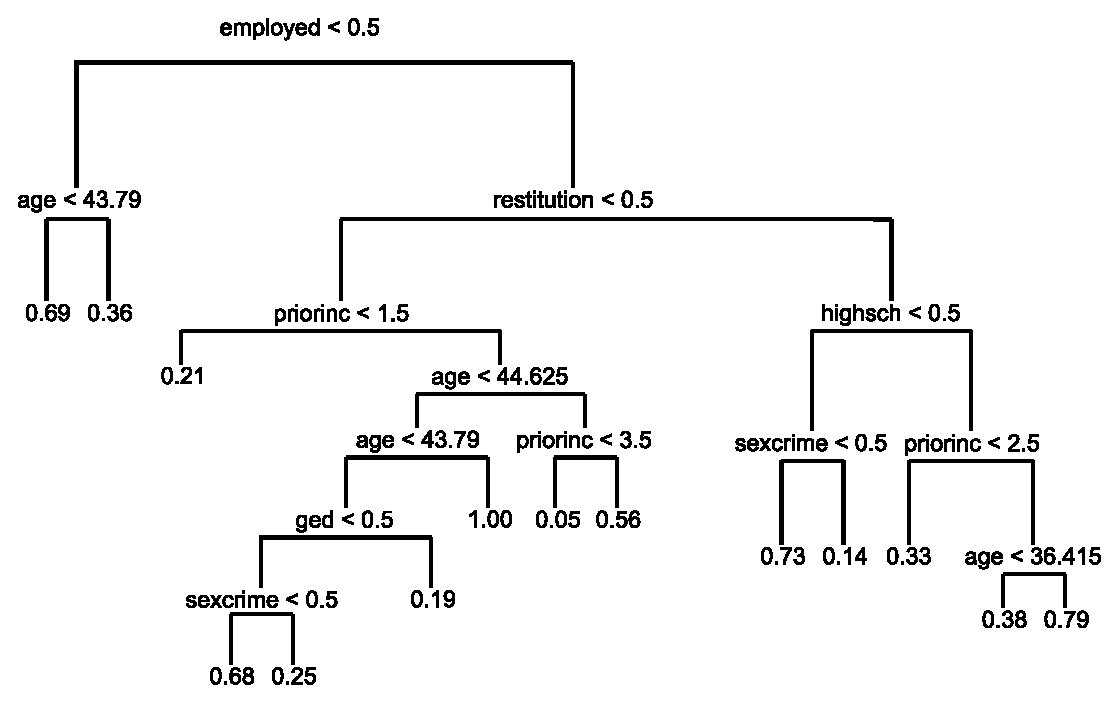
\includegraphics[scale=1]{tree01.eps}
\vspace{0.5cm}
\caption{CART Model 1}
\end{center}
\end{sidewaysfigure}

The selection of variables used for splitting rules in CART Model 1 indicates the importance of these variables to predicting recidivism and the results are generally consistent with the BMA results.  The BMA model indicated that employment, restitution, age at release, and prior incarcerations were the most important predictors of recidivism and all of these variables are present throughout the tree.  The lengths of the branches emanating from the employment and restitution nodes indicate that these two economic variables are among the strongest predictors of recidivism.  Employment status is the splitting rule for the initial node, which shows its importance in separating those predicted to return to prison from those predicted not to return.  With 383 employed parolees classified to the restitution node, the restitution splitting rule acts upon the largest subset of the data.  Of the 383 employed parolees classified to the restitution node, 201 were making restitution payments, which represents 79.4\% of all parolees making restitution payments.  It is interesting to note that while the educational attainment variables GED and high school diploma and the sex offense crime variable were not considered important in the BMA model, they play relatively important roles in the tree model.  This indicates that these variables exhibit nonhomogeneous relationships throughout the range of the entire data set and linear classification methods that operate at the level of the entire data set cannot detect their relationship to recidivism.  When conditionally separated into subsets, all of these variables possess relatively strong relationships to recidivism.

A second tree model, CART Model 2, is presented in Figure 5.4.  The high collinearity between the employment and wage variables ($r=.79$) led the tree modeling process to choose only one of these variables and ignore the other.  CART Model 2 was fitted using the same data set of 506 observations and a total of 36 independent variables, but the wage variable was included and the employment variable was excluded. As expected, the high collinearity between the wage and employment variables led to the substitution of the wage variable for the employment variable at exactly the same location in both tree models.

\begin{sidewaysfigure}
\begin{center}
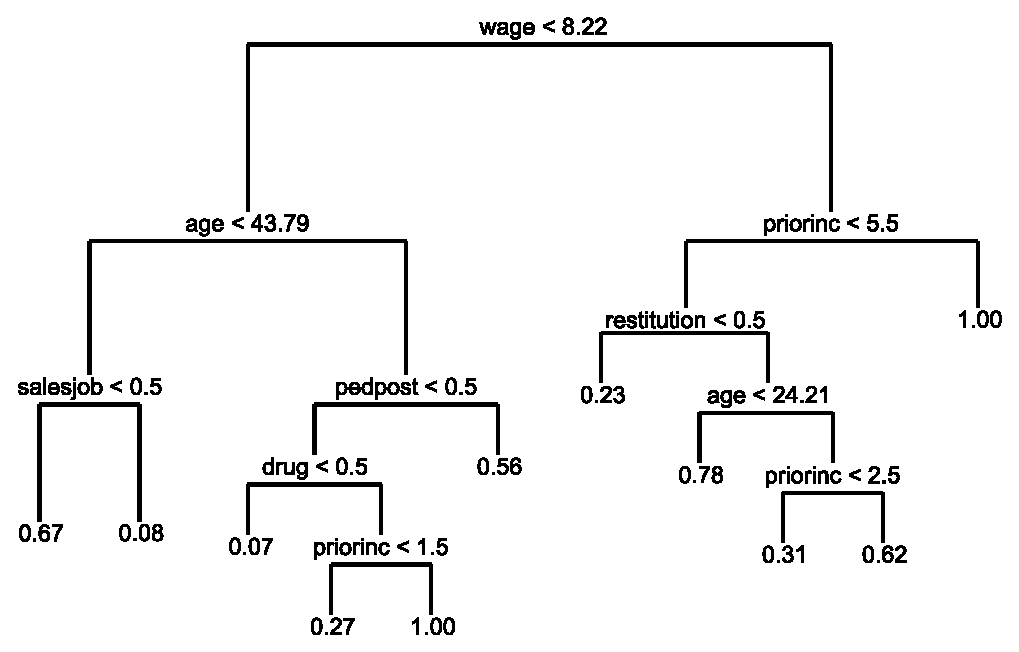
\includegraphics[scale=1]{tree02.eps}
\vspace{0.5cm}
\caption{CART Model 2}
\end{center}
\end{sidewaysfigure}

The two tree models share many similarities.  Consistent with the BMA model and CART Model 1, the variables wage/employment, restitution, age at release, and prior incarcerations all play important roles in CART Model 2.  The restitution variable is still of considerable importance in the second tree model as 257 total observations are classified to the restitution node for further branching.  However, beyond the initial node, there are several structural differences between the two tree models.  The GED, high school diploma, and sex offense variables of CART Model 1 are not present in CART Model 2.  Instead, three new variables are present.  CART Model 2 includes the variables for postsecondary prison education, sales as an occupational type, and drug offense as the most recent crime committed by the parolee.  In the BMA model, none of these variables were important.  The presence of these variables in the tree model implies that these variables exhibit nonhomogeneous relationships and are important predictors of recidivism only within subsets of the entire data set.

The model fit for the second tree model is nearly as good as for the first tree model.  CART Model 2 correctly classified 72.13\% of the observations.  The model predicts that 230 of the 506 parolees will return to prison within three years, which is a recidivism rate of 45.5\%.  Even though the second tree model predicts a recidivism rate that is closer to the actual recidivism rate than the first model, it overestimates the recidivism rate.  On this basis, CART Model 1 might be viewed as preferable for the purpose of risk assessment because arguably a greater injustice occurs from incorrectly classifying nonrecidivists as recidivists than from incorrectly classifying recidivists as nonrecidivists.

\section{A linear probability model}

The last model presented is an OLS linear probability model estimated using the Utah parolee data.  The inclusion of this model is primarily for comparative purposes.  As mentioned previously, over 137 billion different model specifications can be produced from the set of 37 independent variables used to analyze the Utah parolee data.  With such a large number of possible choices, the question arises as to how the particular model specification chosen here was settled upon as being the best model.  The answer, in this case, is simple:  The variable selection was determined by the BMA analysis.  All of the variables included in the regression correspond to the variables that had positive posterior probabilities in the BMA output in Table 5.2.  Besides providing a more familiar set of statistical results for the parolee data, the OLS regression is useful for demonstrating the differences between this classical technique and the two Bayesian techniques.

The OLS regression results for the linear probability model are reported in Table 5.4.  The model correctly classified 66.8\% of the data, which is 2 percentage points greater than the BMA model and 3.7 percentage points less than CART Model 1.  Using the parolee data, it predicts 183 will return to prison, which implies a predicted recidivism rate of approximately 36\%.

\begin{table}[t]
\begin{center}
\caption{Linear Probability Model}
\vspace{0.1cm}
\begin{tabular}{lr@{.}lr@{.}lr@{.}l}
  \hline
   & \multicolumn{2}{c}{Estimate} & \multicolumn{2}{c}{Std. Error} & \multicolumn{2}{c}{$t$ value} \\ \hline
  Intercept \hspace{0.5cm}  & \hspace{0.3cm}  & 760225  & \hspace{0.3cm} & 107300   &  7 & 085 \\
  age	      & $-$ & 005612	&  & 002222 & $-2$ & 526 \\
  priorinc    &     & 046091	&  & 014975 &	3  & 078 \\
  aframer	  &     & 216870	&  & 088010 &	2  & 464 \\
  asian	      & $-$ & 442395	&  & 192963 & $-2$ & 293 \\
  person	  & $-$ & 128181	&  & 062540 & $-2$ & 050 \\
  property    &     & 034771	&  & 054745 &	0  & 635 \\
  sexcrime	  & $-$ & 067588	&  & 060546 & $-1$ & 116 \\
  highsch	  & $-$ & 080350    &  & 047700 & $-1$ & 684 \\
  pedged	  & $-$ & 133274	&  & 051165 & $-2$ & 605 \\
  employed	  & $-$ & 190627	&  & 049320 & $-3$ & 865 \\
  restitution &	    & 094169	&  & 044958 &	2  & 095 \\
  childsup	  &     & 092202	&  & 044803 &	2  & 058 \\
  owncar	  & $-$ & 088958	&  & 043912 & $-2$ & 026 \\
  \hline
\end{tabular}
\normalsize
\end{center}
\end{table}

A comparison of the OLS regression results with the results from the BMA and CART analyses reveals several advantages of the Bayesian methods over the classical method.  First and foremost, both the BMA and CART methods provide solutions to the model specification problem, whereas the OLS linear regression method, in and of itself, is silent on this issue.  Moreover, using the results of an OLS linear regression to determine model specification may lead to the selection of the wrong variables.  Referring to Table 5.4, a researcher using a stepwise elimination approach may decide to reject the property crime, sex crime, and possibly the high school diploma variables due to their relatively low $t$ statistics.  However, both the BMA and CART methods indicate that these variable have a role to play in predicting recidivism.  In the BMA results in Table 5.2, the posterior probabilities associated with the property crime, sex crime, and high school diploma variables were 33\%, 3.6\%, and 3.5\%, respectively.  While these low probabilities indicate that these variables are somewhat weak predictors, it seems better to include them rather than omit them completely.  CART Model 1 adds further evidence that at least two of these variables play a significant role in prediction.  The high school diploma variable is used to separate out 201 observations and the two occurrences of the sex crime variable together separate out 93 observations, which indicates that these variables are relevant for predicting recidivism.  In their different ways, the CART and BMA approaches find these variables important while the OLS linear regression model does not.

Another issue than can be illustrated by way of these comparisons concerns the estimated magnitude of the coefficients.  The OLS estimates in Table 5.4 for age, prior incarcerations, and employment status are very similar to the BMA estimates of -.005, .045, and -.2, respectively.  This results from the facts that the BMA posterior probabilities are very high for these variables and that the OLS estimation procedure effectively assumes these variables are certainly members of the best model.  As for the other variables, the magnitudes of the OLS coefficients are quite different as compared to the BMA expected values.  BMA adjusts the size of the coefficients to reflect the uncertainty expressed in the posterior probabilities for each variable.  Consequently, OLS produces coefficients that are too large because it assumes the variables all belong to the best model.  In a sense, OLS estimation leads to a different type of over-fitting problem, one stemming from its inability to incorporate uncertainty about the variables into the estimation procedure.  Similar to the problem of over-fitting as the term is used in its ordinary sense, the OLS model can be expected to perform worse on out-of-sample predictions in comparison to the BMA model.

\section{A summary of the results}

The analyses reveal that there are seven variables that are of particular importance to predicting recidivism.  Among the economic variables, employment status, restitution payments, and child support payments are the most important.  As for the sociological variables, age, prior incarcerations, and the Asian and African American race variables were the strongest predictors.  Together, the BMA and CART models clearly show that the four most powerful predictors are employment, age, prior incarcerations, and restitution.

In comparison with past recidivism studies, the importance of the variables age, race, prior incarcerations, and crime type as found in the Utah parolee data set is consistent with past results.  The gender, education, and Hispanic race variables were found to be unimportant in the Utah parolee data set, which generally conforms to the results from past studies.  Even though wages were removed from the BMA model due to high collinearity with employment, wages were found to be significantly related to recidivism in the Utah parolee data set, which is consistent with the past studies. However, the relationship between employment status and recidivism was found to be of uncertain significance in previous studies and it is the single-most important variable in the parolee data set.  Restitution payments, which exhibited a somewhat weak negative relationship with recidivism in earlier research, showed a strong positive relationship.  Finally, job type was found to be related to recidivism in past studies, but no significant relationship was found in the Utah data set.

The 10-fold cross-validation showed that economic variables are just slightly better predictors of recidivism than sociological variables.  The Total Model, composed of both economic and sociological variables, performed even better, indicating that the best model would incorporate a mix of these variables.

Regarding model fit, the BMA model correctly classified 64.8\% of Utah parolees, while the OLS linear probability model correctly classified 66.8\%.  The tree methodology developed models that fit the data much better than either the BMA or OLS models.  CART Model 1 correctly classified 72.5\% of the parolees and CART Model 2 correctly classified 72.1\%.

